\documentclass[11pt,aspectratio=169]{beamer}
\usepackage[utf8]{inputenc}
\usepackage[T1]{fontenc}
\usepackage{lmodern}
\usepackage{amsmath}
\usepackage{amsfonts}
\usepackage{amssymb}
\usepackage{graphicx}
\usepackage{hyperref}
\usepackage{listings}
\usepackage{xcolor}

\definecolor{codegreen}{rgb}{0,0.6,0}
\definecolor{codegray}{rgb}{0.5,0.5,0.5}
\definecolor{codepurple}{rgb}{0.58,0,0.82}
\definecolor{backcolour}{rgb}{0.95,0.95,0.92}

\lstdefinestyle{standard}{
	backgroundcolor=\color{backcolour},   
	commentstyle=\color{codegreen},
	keywordstyle=\color{magenta},
	numberstyle=\tiny\color{codegray},
	stringstyle=\color{codepurple},
	basicstyle=\ttfamily\tiny,
	breakatwhitespace=false,         
	breaklines=true,                 
	captionpos=b,                    
	keepspaces=true,             
	numbersep=5pt,                  
	showspaces=false,                
	showstringspaces=false,
	showtabs=false,                  
	tabsize=4
}
\lstset{style=standard}

\usetheme{Singapore}
\begin{document}
	\author{Quan Gan}
	\title{Introduction to DGL}
	%\subtitle{}
	%\logo{}
	\institute{AWS Shanghai AI Lab}
	%\date{}
	%\subject{}
	%\setbeamercovered{transparent}
	\setbeamertemplate{navigation symbols}{}
	\begin{frame}[plain]
		\maketitle
	\end{frame}
	
	\begin{frame}
		\frametitle{Recap: Graph Neural Networks}
		$$
		h^{(k)}_v = \phi\left(
		h^{(k-1)}_v,
		h^{(k)}_{\mathcal{N}(v)}
		\right) \qquad h^{(k)}_{\mathcal{N}(v)} = f\left(
		\left\lbrace
		h^{(k-1)}_u : u \in \mathcal{N}(v)
		\right\rbrace
		\right) \footnote{Xu et al., \emph{How Powerful Are Graph Neural Networks?}, ICLR 2019}
		$$
		\begin{center}
			\centering
			\only<1>{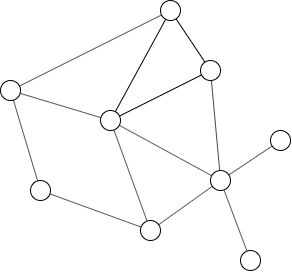
\includegraphics[width=0.4\textwidth]{graph-1.png}}
			\only<2>{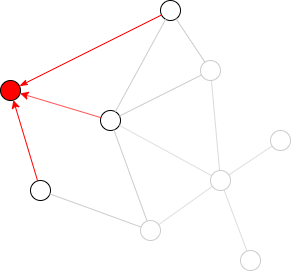
\includegraphics[width=0.4\textwidth]{graph-2.png}}
			\only<3>{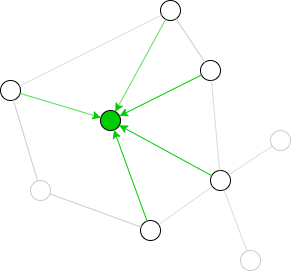
\includegraphics[width=0.4\textwidth]{graph-3.png}}
			\only<4>{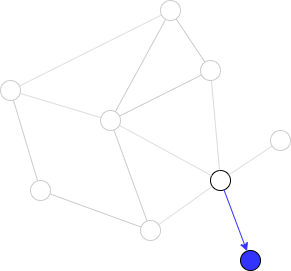
\includegraphics[width=0.4\textwidth]{graph-4.png}}
		\end{center}
	\end{frame}

	\begin{frame}[fragile]
		\frametitle{A common case\footnote{Hamilton et al., \emph{Inductive Representation Learning on Large Graphs}, NIPS 2017}}
		\begin{minipage}{0.4\textwidth}
		If $f(\cdot)$ is summation:
		$$
		\begin{gathered}
		h_{\mathcal{N}(v)}^{(k)} =
		\sum_{u \in \mathcal{N}(v)} h^{(k-1)}_u \\
		h^{(k)}_v =
		\sigma \left( W^{(k)} \left[h_v^{(k-1)} \Vert h_{\mathcal{N}(v)}^{(k)}\right] \right)
		\end{gathered}
		$$
		\end{minipage}\hfill%
		\begin{minipage}{0.5\textwidth}
			Sparse matrix multiplication, easy:
\begin{lstlisting}[language=Python]
# code: PyTorch
# src: edge source node IDs (n_nodes,)
# dst: edge destination node IDs (n_nodes,)
# H: node repr matrix (n_nodes, in_dim)
# W: weights (in_dim, out_dim)
A = torch.sparse_coo_tensor(
    torch.stack([dst, src], 0),
    torch.ones(n_nodes),
    (n_nodes, n_nodes)
    )
H_N = A @ H
H = torch.relu(H_N @ W)
\end{lstlisting}
		\end{minipage}
	\end{frame}

	\begin{frame}[fragile]
		\frametitle{How about max pooling?}
		
		\begin{minipage}{0.4\textwidth}
			If $f(\cdot)$ is summation:
			$$
			\begin{gathered}
			h_{\mathcal{N}(v)}^{(k)} =
			\sum_{u \in \mathcal{N}(v)} h^{(k-1)}_u \\
			h^{(k)}_v =
			\sigma \left( W^{(k)} \left[h_v^{(k-1)} \Vert h_{\mathcal{N}(v)}^{(k)}\right] \right)
			\end{gathered}
			$$
		\end{minipage}\hfill%
		\begin{minipage}{0.5\textwidth}
			Only Tensorflow supports what we need natively:
\begin{lstlisting}[language=Python]
# code: Tensorflow
# src: edge source node IDs (n_nodes,)
# dst: edge destination node IDs (n_nodes,)
# H: node repr matrix (n_nodes, in_dim)
# W: weights (in_dim, out_dim)
H_src = H[src]    # broadcast to edges
H_N = tf.unsorted_segment_max(H_src, dst, n_nodes)
H = torch.relu(H_N @ W)
\end{lstlisting}
		\end{minipage}
	\end{frame}

	\begin{frame}[fragile]
		\frametitle{With attention?\footnote{Velickovic et al., \emph{Graph Attention Networks}, ICLR 2018}}
		\begin{minipage}{0.4\textwidth}
			If $f(\cdot)$ is summation:
			$$
			\begin{gathered}
			\hat\alpha ^{(k-1)}_{v,u} = MLP\left(\left[h_v^{(k-1)} \Vert h_u^{(k-1)}\right]\right) \\
			\alpha^{(k-1)}_{v,u} = softmax_j\left(
			\hat\alpha ^{(k-1)}_{v,u}
			\right)\\
			h_{\mathcal{N}(v)}^{(k)} =
			\sum_{u \in \mathcal{N}(v)} \alpha^{(k-1)}_{v,u} h^{(k-1)}_u \\
			h^{(k)}_v =
			\sigma \left( W^{(k)} \left[h_v^{(k-1)}; h_{\mathcal{N}(v)}^{(k)}\right] \right)
			\end{gathered}
			$$
		\end{minipage}\hfill%
		\begin{minipage}{0.5\textwidth}
			Can't do it easily with PyTorch/MXNet.  Possible in Tensorflow
			\begin{lstlisting}[language=Python]
# code: Tensorflow
# src: edge source node IDs (n_nodes,)
# dst: edge destination node IDs (n_nodes,)
# H: node repr matrix (n_nodes, in_dim)
# W: weights (in_dim, out_dim)
# U: attention MLP weights (in_dim * 2)
			\end{lstlisting}
		\end{minipage}
	\end{frame}

	\begin{frame}
		Attention
		
		Need both.
	\end{frame}

	\begin{frame}
		LSTM?
		
		Need to manually pad the neighbors into the same length.
	\end{frame}

	\begin{frame}
		As long as a model can be expressed as message passing, DGL can handle it
		without changing much of your code.
		
		[TODO: four cases]
	\end{frame}

	\begin{frame}
		Scaling to larger graphs.
	\end{frame}
\end{document}